\section{Estudo de Caso}

% Reafirmar o objetivo
O modelo de referência descrito na seção anterior, fruto da iniciativa de BI do Tribunal Regional do Rio Grande do Norte ainda não foi massivamente disponibilizado para os servidores da instituição até o momento da escrita deste trabalho. Logo, a carga ao qual os serviços que compõem o modelo de referência ainda não é tão elevada, não apresentando muitos momentos de degradação de performance.

No entanto, durante o ano de 2019, ocorreram alguns eventos de divulgação e repasse dos trabalhos desenvolvidos pela residência de TI, onde poderam-se observar momentos de carga não habitual, principalmente no serviço de visualização de dados, o Metabase.

Um destes momentos foi um treinamento de cerca de 60 servidores de diversos Tribunais da Justiça Eleitoral brasileira que vieram a sede do TRE-RN, onde foram ministrados dois dias de conteúdo prático de desenvolvimento de aplicações de dados utilizando-se o modelo de referência. Os efeitos sentidos pelos servidores convidados foram basicamente a indisponibilidade do serviço ou tempo de resposta maior que o habitual. Infelizmente, as estatíscas de consumo da instância do Metabase que foi utilizada para este treinamento não foram salvas, por se tratar de uma instância criada com o único objetivo de realização do evento. 

Para que possamos quantificar o impacto do cenário descrito, tentou-se simular a carga a qual o Metabase foi exposto. A ferramenta utilizada para a simulação foi o \textit{Apache HTTP server benchmarking}, utilizando um \textit{MacBook Pro Mid 2014} equipado com processador Intel Core i5-4278U, 8GB de RAM DDR3 e rodando o sistema macOS Mojave versão 10.14.6. O serviço do Metabase foi hospedado no mesmo modelo descrito na Figura \ref{fig:arq_metabase}, utilizando containeres \textit{Docker}. 

O cenário de teste consiste em multiplos usuários realizando autenticação no serviço, com a quantidade usuários simultâneos variando de 1 a 60, em passos de 10 usuários. Foram realizados um total de 200 requisições para cada quantidade de usuário simultâneos. 

A Figura \ref{fig.avg-resp-time} apresenta o tempo médio de resposta do Metabase para cada cenário testado. Nos resultados apresentados podemos observar que o tempo médio de resposta cresce a uma taxa quase linear a quantidade de usuários simultâneos. Este aumento será percebido pelos usuários na demora do sistema ao carregar as telas, gerando um experiência de uso não satisfatória. 

\begin{figure}[htp]
   \centering
    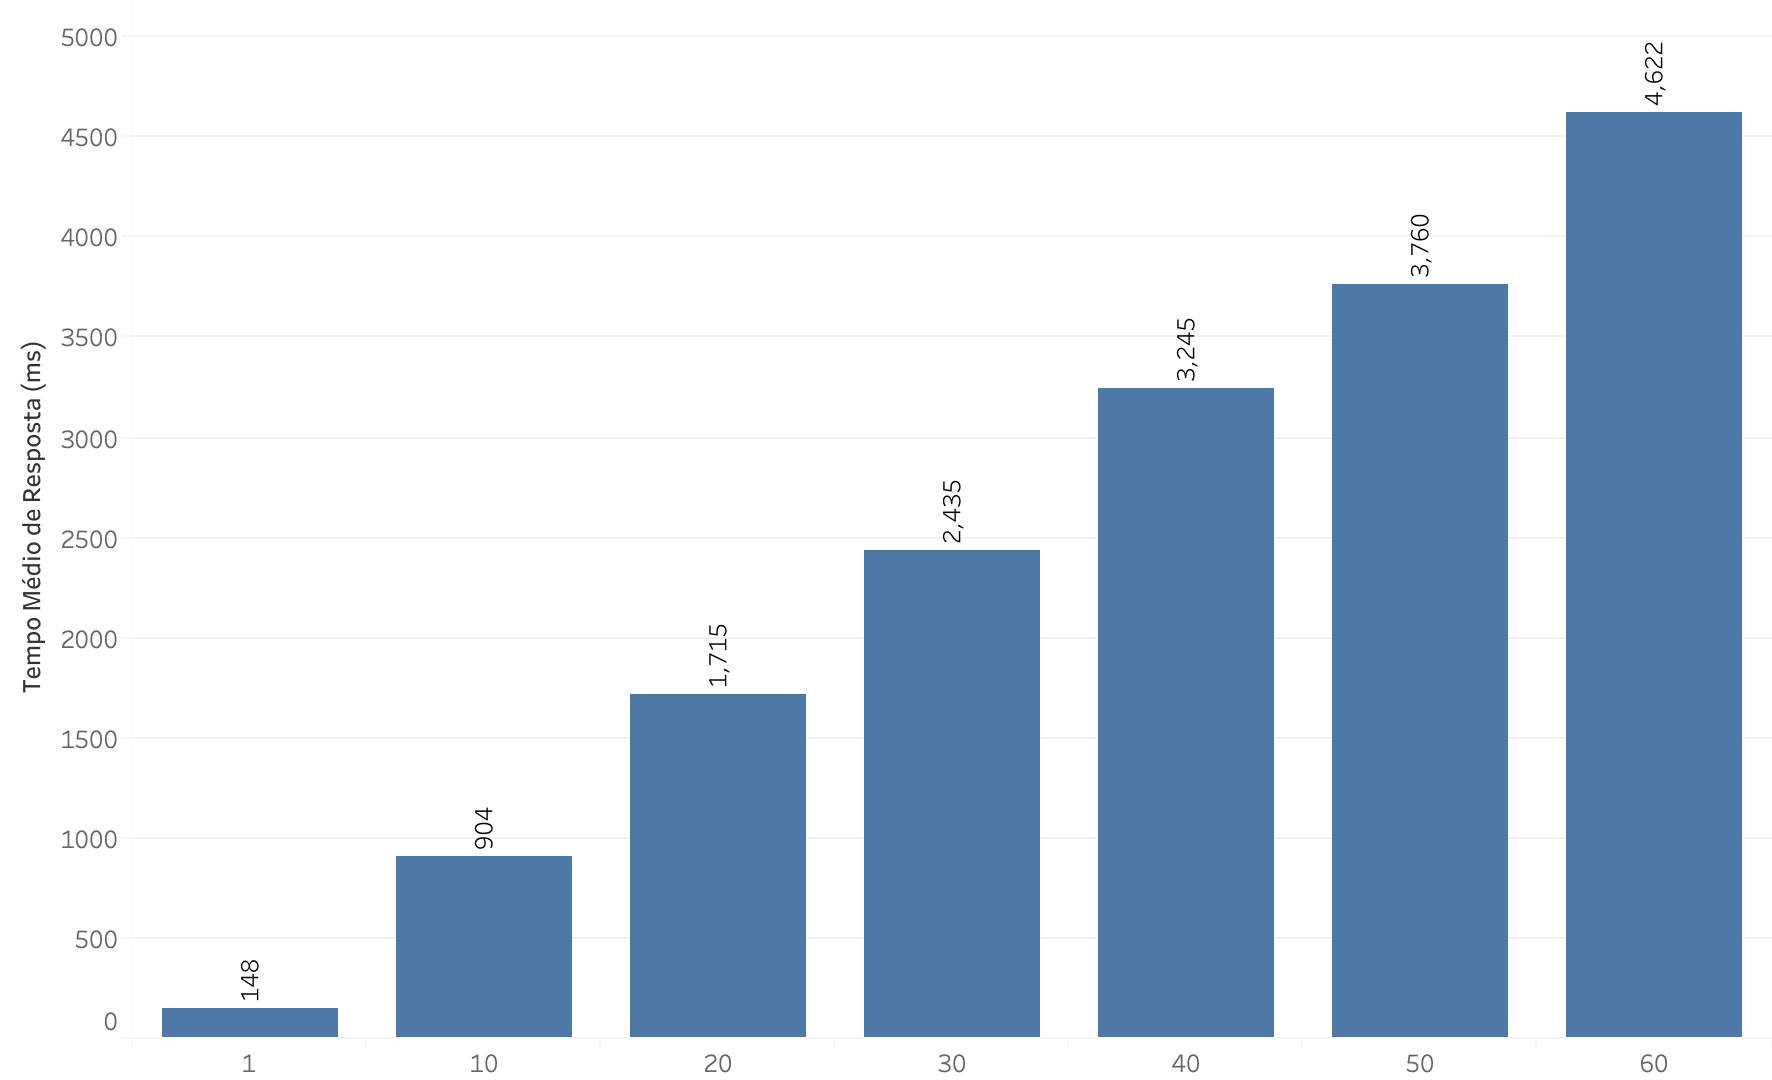
\includegraphics[width=8cm]{Imagens/avg-response-time}
    \caption{Tempo Médio de Resposta de Autenticação para Instância Única.}
    \label{fig.avg-resp-time}
\end{figure} 

A próxima seção deste trabalho irá descrever o procedimento do hospedagem do Metabase em um modelo de multiplas instâncias com escalabilidade automática, utilizando o \textit{Kubernetes} como osquestrador dos containeres \textit{Docker}.

